 \providecommand{\main}{../../..}
\documentclass[\main/main.tex]{subfiles}
\begin{document}
\subsection{Esercizio 1}
Dato il seguente problema di PL:

\begin{figure}
  \begin{align*}
    \max z = x_1 -3x_2  \\
    x_1 + x_2  & \leq 7 \\
    x_2        & \leq 5 \\
    x_1 + 2x_2 & \geq 2 \\
    x_1 - x_2  & \leq 0 \\
    x_1, x_2   & \geq 0
  \end{align*}
  \caption{Esercizio 1}
\end{figure}

\begin{enumerate}
  \item Si disegni la regione ammissibile e si evidenzi il vertice ottimo per via grafica, riportando il valore di z e di tutte le variabili del modello, comprese quelle di scarto.
  \item Si ricavi per via grafica per quali valori di $b_3$, ora pari a $2$, la \textbf{composizione} della base ottima non cambia.
  \item Si risolva mediante gli scarti complementari il duale del problema.
\end{enumerate}

\subsection{Soluzione esercizio 1}

\subsubsection*{Identifico soluzione ottima}

\begin{figure}
  \begin{subfigure}{0.49\textwidth}
    \dddgraph{x_2}{x_1}{0}{5}{0}{4}{-17}{
      x + y   <= 7 &&
      x         <= 5 &&
      y + 2*x  >= 2 &&
      y - x   <= 0}{y -3*x}
    \caption{Il vertice ottimo ha coordinate $\bmx = \rnd{\frac{2}{3},\frac{2}{3}}$}
  \end{subfigure}
  \begin{subfigure}{0.49\textwidth}
    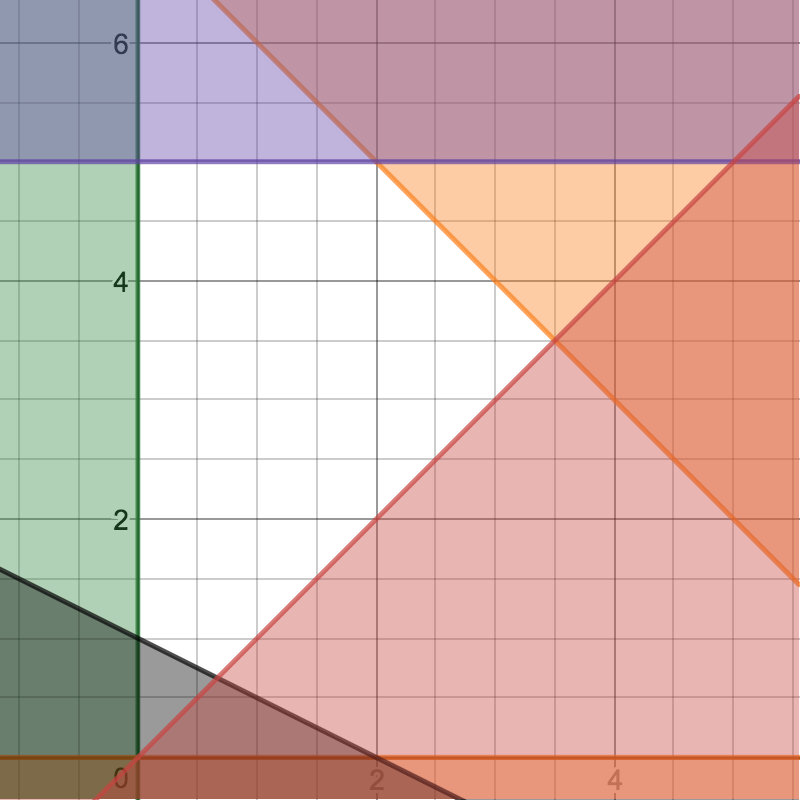
\includegraphics[width=0.9\textwidth]{2014_07_03}
    \caption{Regione di ammissibilità del problema}
  \end{subfigure}
  \caption{Vertice ottimo del problema di massimo}
\end{figure}

\subsubsection*{Riporto variabili}

\begin{align*}
  z = -\frac{4}{3}, \quad
  x_1 = \frac{2}{3}, \quad
  x_2 = \frac{2}{3}, \quad
  s_1 = \frac{17}{3}, \quad
  s_2 = \frac{13}{3}, \quad
  s_3 = 0, \quad
  s_4 = 0
\end{align*}
\subsubsection*{Analisi di sensitività}
La variabile $b_3$ può variare tra $0$, valore in cui il vincolo incrocia il vertice $(0,0)$ e $\frac{21}{2}$, valore in cui incrocia il vertice in $\rnd{\frac{3}{2}, \frac{3}{2}}$.

\begin{figure}
  \begin{subfigure}{0.49\textwidth}
    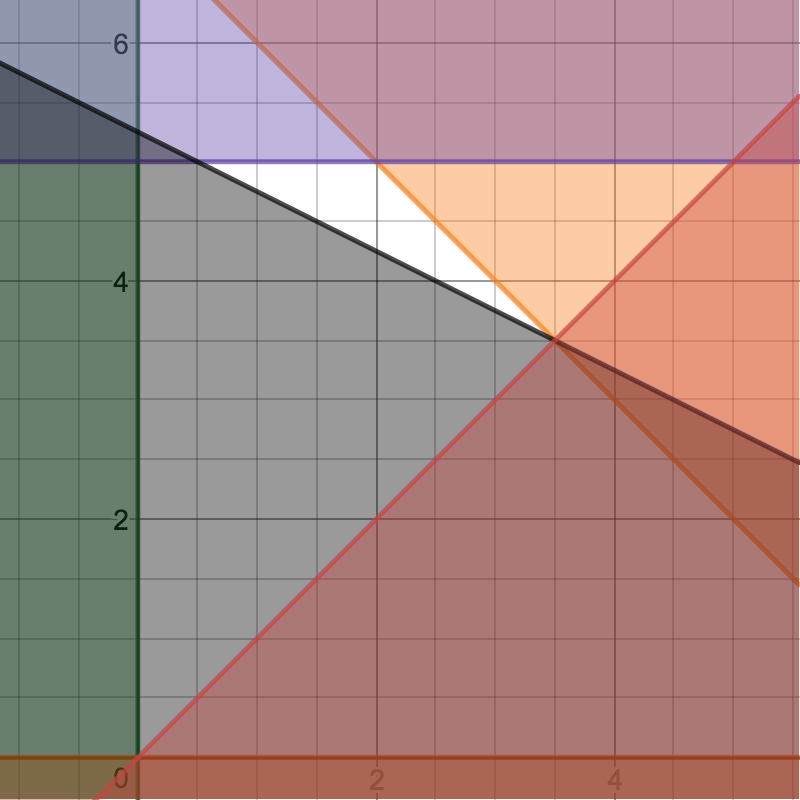
\includegraphics[width=0.9\textwidth]{2014_07_03_1}
    \caption{$b_3 = \frac{21}{2}$}
  \end{subfigure}
  \begin{subfigure}{0.49\textwidth}
    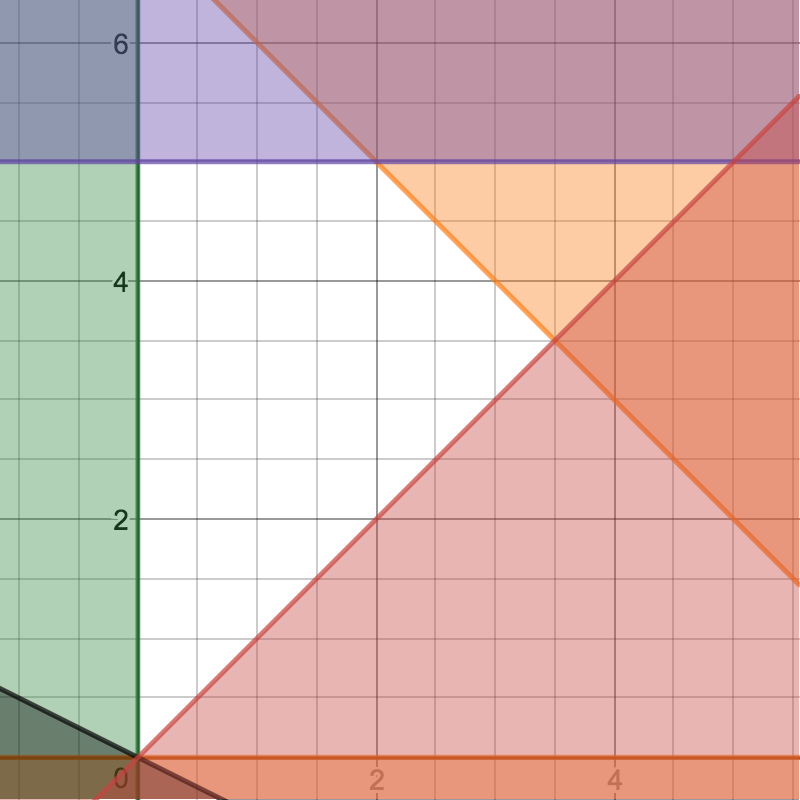
\includegraphics[width=0.9\textwidth]{2014_07_03_2}
    \caption{$b_3 = 0$}
  \end{subfigure}
  \caption{Analisi di sensitività}
\end{figure}

\subsubsection*{Costruisco problema duale}
\begin{align*}
  \min z_D = 7y_1 + 5y_2 + 2y_3   \\
  y_1 + y_3 + y_4       & \geq 1  \\
  y_1 + y_2 + 2y_3 -y_4 & \geq -3 \\
  y_1, y_2, y_4         & \geq 0  \\
  y_3                   & \leq 0
\end{align*}
\subsubsection*{Scarti complementari}
\[
  \begin{cases}
    x_1(y_1 + y_3 + y_4       - 1 )=0 \\
    x_2(y_1 + y_2 + 2y_3 -y_4 +3)=0   \\
    y_1(x_1 + x_2 - 7) = 0            \\
    y_2(x_2       - 5) = 0            \\
    y_3(x_1 + 2x_2- 2) = 0            \\
    y_4(x_1 - x_2 - 0) = 0            \\
  \end{cases}
  \Rightarrow
  \begin{cases}
    y_3 + y_4 - 1 =0 \\
    2y_3 -y_4 +3=0   \\
    y_1 = 0          \\
    y_2 = 0          \\
  \end{cases}
  \Rightarrow
  \begin{cases}
    y_3 =-\frac{2}{3} \\
    y_4=\frac{5}{3}   \\
    y_1 = 0           \\
    y_2 = 0           \\
  \end{cases}
\]
Verifico che la soluzione ottima del duale corrisponda a quella del primale: $z = z_D = -\frac{4}{3}$.
\end{document}